\documentclass{llncs}
\usepackage{epsfig}
\usepackage{graphicx}

\newtheorem{mydef}{Def.}
\newtheorem{myhyp}{Hypothesis}

\usepackage{url}
\usepackage{hyperref}
\usepackage{cleveref}
\usepackage{hhline}
\usepackage{caption}
\usepackage{subcaption}

%\pagestyle{empty}
\pagestyle{headings} 

\begin{document}

% ====================================================================
       
\title{Using Metric Space Indexing for Complete and Efficient Record Linkage}

% ====================================================================

\author{Submitted for double-blind review}

%  Hidden For Blind Review
\iffalse  

\author{{\"O}zg{\"u}r Akg{\"u}n\inst{1} \and Alan Dearle\inst{1} \and\\
Graham Kirby\inst{1} \and Peter Christen\inst{2}}

\institute{School of Computer Science, University of St Andrews,\\
St Andrews, Scotland. Contact: \email{ozgur.akgun@st-andrews.ac.uk}
\and
Research School of Computer Science, The Australian National University,\\
Canberra, Australia. Contact: \email{peter.christen@anu.edu.au}}
      
\fi
% ====================================================================

\maketitle

\begin{abstract}

Record linkage is the process of identifying records that refer to the
same real-world entities, in situations where entity identifiers are
unavailable. Records are linked on the basis of similarity between
common attributes, with every pair of records being classified as a
link or non-link depending on the degree of similarity between them.
Record linkage is usually performed in a three-step process: first
groups of similar candidate records are identified using indexing; 
pairs within the same group are then compared in more detail, and
finally classified.
%
Even state-of-the-art indexing techniques, such as Locality Sensitive
Hashing, have potential drawbacks. They may fail to group together some
true matching records with high similarity. Conversely, they may group
records with low similarity, leading to high computational overhead.
%
We propose using metric space indexing to perform \emph{complete} record
linkage, which results in a parameter-free record linkage process
combining indexing, comparison and classification into a single step
delivering complete and efficient record linkage.

\end{abstract}

\keywords Entity resolution; data matching; similarity search;
         blocking.

% ====================================================================

\section{Introduction}
\label{sec-intro}

Record linkage, also known as entity resolution, data matching and
duplicate detection~\cite{Chr12}, is the process of identifying and
matching records that refer to the same real-world entities within or
across datasets. The entities to be linked are often people (such as
patients in hospital or customers in business datasets), but record
linkage can also be applied to link consumer products or bibliographic
records~\cite{Chr12}. Record linkage is commonly challenged by the lack
of unique entity identifiers (keys) in the datasets to be linked, which
prevents the use of a database join. Instead, the linkage of records
requires the comparison of the common attributes (or fields) that are
available within the datasets. For datasets that contain information
about individuals, these attributes include the names, address, dates of
birth, and so on, of individuals.

To overcome data quality issues such as typographical errors and
variations (which are common in name and address values~\cite{Chr12}),
approximate string comparison functions (such as edit distance, the
Jaro-Winkler comparator, or Jaccard similarity~\cite{Chr12}) are used to
compare pairs of records, leading to a vector of similarities (one
similarity per attribute/field compared) for each pair. These similarity
vectors are then used to classify the compared record pairs into links
(where it is assumed both records in a pair correspond to the same
real-world entity) and non-links (where the records are assumed to
correspond to two different entities). Various classification methods
have been employed in record linkage~\cite{Chr12,Don15}, ranging from
simple threshold-based to sophisticated clustering, supervised
classification techniques, and active learning approaches~\cite{Wan15}.

Besides the issues of a lack of unique entity identifiers, and data
quality (which will affect linkage quality), record linkage is also
challenged by the increasing sizes of the datasets to be
linked~\cite{Don15}. To avoid full pair-wise comparison of all possible
record pairs (quadratic in the sizes of the datasets to be linked),
blocking techniques, commonly known as \emph{indexing}~\cite{Chr12b},
are used. These split the datasets into smaller blocks in a
computationally efficient way, such that records that are likely to
correspond to the same entity are grouped into the same block. Only
records within the same block are then compared in more detail.

While indexing techniques facilitate efficient linkage of very large
datasets~\cite{Don15}, they generally achieve scalability at the cost
of reduced linkage quality, because potentially true matching record
pairs are removed in the indexing step, leading to a reduction in recall
of the final linkage result~\cite{Chr12}. A variety of indexing
techniques, discussed in more detail in the following section, have
been proposed, ranging from simple phonetic based blocking~\cite{Chr12}
and sorting of the datasets~\cite{Dra12} to locality sensitive hashing
based techniques~\cite{Kim10,Steorts2014}. Techniques for
unsupervised~\cite{Kej13,Ram15} and supervised~\cite{Bil06,Mic06}
learning of optimal blocking schemes have also been proposed.

\begin{figure}[!t]
  \centering
  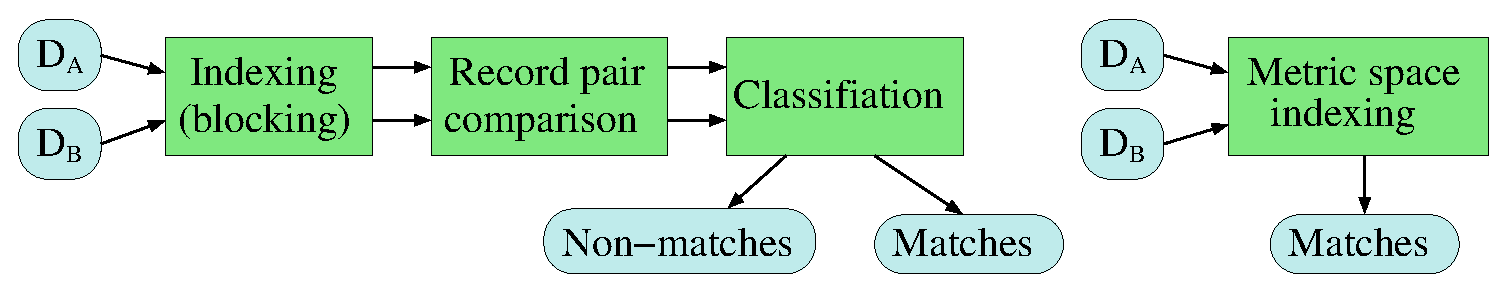
\includegraphics[width=1.0\textwidth]{figures/linkage-process}
  \caption{Overview of the steps of the traditional record linkage
           process (left-hand side) and our proposed metric space
           indexing based approach (right-hand side), as described in
           Sect.~\ref{sec-intro}, where records from two datasets,
           $\mathbf{D}_A$ and $\mathbf{D}_B$, are being linked.}
           \label{fig-rl-process}
\end{figure}

Systems that perform indexing prior to comparison and classification, as
illustrated in Fig.~\ref{fig-rl-process}, add a further practical
complexity to the process. Indexing, comparison and classification are
often conducted using algorithms and parameters selected based on
technical and domain expertise of the user of the record linkage system,
followed by a manual assessment (auditing) of the linkage
outcomes~\cite{Chr12}. If the quality of the resulting links is not good
enough for a certain application, the linkage process needs to be
repeated with different parameter settings and possibly also alternative
algorithms. This can result in a time-consuming and labour-intensive
iterative process. A major challenge is often the heuristic nature of
indexing, where the choice of a certain indexing technique and its
parameters (including which attributes to use in indexing) will
determine the final outcome of a linkage.

This paper focuses on approaches that use a similarity threshold to
classify links. Such techniques are fundamentally limited by the extent
to which true matching records are similar, and true non-matches are
dissimilar---this is dataset-dependent. Within this domain, we define
a technique to be \emph{complete} if it is guaranteed to identify all
pairs within the specified similarity threshold. Commonly used indexing
techniques are incomplete, since they reduce computational cost at the
expense of potentially overlooking some true matches. By definition,
incomplete techniques yield lower recall than complete techniques.
Conversely, and perhaps counter-intuitively, complete techniques can
yield lower precision with some datasets. This is discussed further in
Sect.~\ref{sec-approach}.

\emph{Metric space indexing} (MSI) is a complete technique with much
lower computational overheads than a brute-force approach. It allows
indexing, comparison and classification to be combined into a single
step, as shown in Fig.~\ref{fig-rl-process}, making the overall record
linkage process simpler, more efficient and more effective than
incomplete indexing approaches.

\textbf{Contribution:} the primary contribution of this paper is the
novel application of MSI to achieve complete and efficient record
linkage, without the need for complex parameter tuning. We evaluate our
approach on several datasets from diverse domains and demonstrate its
advantages over existing indexing techniques for record linkage.

% For final paper:
% The motivation for this work is the Digitising Scotland project
% (Dibben 2012), which is in the process of transcribing and linking all
% the vital events recorded in Scotland between 1856 and 1977. This data
% set will, when complete, include around 14 million birth records, 11
% million death records and 4 million marriage records. As part of the
% work, certain data fields (locations, occupations and causes of death)
% are also being classified to the relevant standard coding schemes.

% --------------------------------------------------------------------

\section{Related Work}
\label{sec-related}

We now briefly review relevant work in the areas of indexing for record
linkage (for recent surveys see~\cite{Chr12b,Pap16}), and metric space
indexing~\cite{Zezula2010}.

Techniques to link records across datasets have been investigated for
over five decades~\cite{Fel69,New59}, with the scalability of linking
being an ongoing challenge as datasets grow in size and complexity.
Traditional blocking~\cite{Chr12b} uses a set of attributes (known as a
\emph{blocking key}) to insert records that share the same value(s) in
their blocking key into the same block. Only records within the same
block are  compared to each other. To overcome variations and
misspellings, the values used in blocking keys can be phonetically
encoded using functions such as Soundex, NYSIIS, or
Double-Metaphone~\cite{Chr12}. These convert a string into a code
according to its pronunciation, assigning the same code to similar
sounding names (such as `Gail' and `Gayle'). Multiple blocking keys may
be used to deal with the problem of missing attribute values.

A different approach to indexing is the sorted neighbourhood
method~\cite{Mon96}, where the datasets to be linked are sorted
according to a \emph{sorting key} (usually a concatenation of the values
from several attributes). A sliding window is then moved over the
datasets and only records within the window are compared. Techniques
that adaptively shrink or expand the window size based on the
characteristics of the sorting key values have shown to improve both
linkage efficiency and quality~\cite{Dra12} over other sliding window
approaches.

These blocking techniques are heuristics, commonly requiring domain
knowledge, such as the choice of appropriate blocking or sorting keys.
Poor choices of blocking attributes result in records being inserted
into inappropriate blocks, and thus true matches being missed. As a
result, such techniques can lead to \emph{incomplete} linkage.
Conversely, many of the record pairs compared in a block may turn
out to have low similarity, corresponding to non-matches, resulting in
\emph{inefficient} linkage.

Locality sensitive hashing (LSH), originally proposed to allow efficient
nearest-neighbour search in high-dimensional spaces~\cite{Ind98}, has
been employed in record linkage as an indexing technique where attribute
values are hashed multiple times, and blocks are created from those
records that share some hash values. \emph{HARRA}~\cite{Kim10} is a
record linkage approach based on MinHash~\cite{Broder1997} and LSH which
blocks, compares, and then merges linked records in an iterative
fashion, where merged records are re-hashed to improve overall linkage
quality. ~\cite{Steorts2014} evaluates two LSH variations, concluding
that in order to get good results, LSH methods must be tuned to the
particular datasets being linked. This requires good quality ground
truth data which may be unavailable or expensive to obtain.

Metric space indexing (MSI) techniques provide indexing structures to
support the comparison of records in one set with those in another,
typically also offering similarity search operations. To create an MSI
data structure, it is necessary to define a distance measure between
records, with certain properties including the \emph{triangle
inequality}. Similarity search operations include
\textit{range-search(q,d)}, where all records within a distance $d$ of a
query record $q$ are identified; \textit{nearest-neighbour(q)},
returning the record with smallest distance to $q$; and
\textit{nearest-n(q,n)}, returning the $n$ closest records to $q$.
\cite{Zezula2010} gives an overview of MSI techniques.
Here we choose one metric space indexing structure, the M-tree
\cite{paolociaccia2m}, and investigate its efficacy for record linkage.

The M-tree is a dynamically balanced tree structure. Every node contains
a reference to a record being indexed, a pointer to its parent, the
distance to its parent, and the node's radius. The radius of a node is
the distance from it to its furthest child. For a parent node with
radius \textit{r}, all its children may be visualised as being contained
within a ball of radius \textit{r} from it.

\cite{Li2006} describes a threshold-based linkage method using
R-trees~\cite{Hjaltason1998}. It demonstrates that high quality may be
achieved using Jaccard similarity over selected record fields.
\cite{Ciaccia97indexingmetric} shows that M-trees are almost always more
efficient than R-trees, hence their use in the experiments described in
this paper.

% --------------------------------------------------------------------

\section{Approach}
\label{sec-approach}

We address the following general record linkage problem: for two
datasets $A$ and $B$, we wish to find, for each record in $A$, all the
records in $B$ that match it. We compare several algorithms for record
linkage: traditional blocking, one incomplete similarity search method,
LSH-MinHash, and one complete method, M-tree~\cite{paolociaccia2m}. We
also use a simple complete brute-force technique as a baseline for
comparison, although this can only feasibly be applied to the smallest
of our datasets. All experiments have a number of parameters to
configure the search space and algorithm behaviour, including a
\emph{distance threshold} specifying a maximum distance, equivalent to a
minimum similarity, for two records to be classified as a link (i.e.\
referring to the same entity).

\textbf{Brute-force:}
Two nested loops are used to compare every record in $A$ with every
record in $B$. Each pair is classified as a link if the distance between
the records is less than the threshold. This approach is guaranteed to
identify all links, with complexity $ O(|A| \times |B|) $.

\textbf{Traditional blocking:}
The additional parameters are the set of blocking keys and the
normalization encodings applied to each field. These are selected as
described in \cite{Chr12b}, exploiting knowledge of the domain and of
the records being linked, and chosen with the intention of giving the
best possible results for the datasets. Each record in $A$ is placed
into the appropriate block based on its blocking key value. The
algorithm then iterates over the records in $B$, and for each one,
compares it with each of the records from $A$ in the block with the same
blocking key value.

\textbf{LSH-MinHash:}
The additional parameters are \emph{shingle size} ($l_{ss}$), \emph{band
size} ($l_{bs}$) and \emph{number of bands} ($l_{nb}$). Each record in
$A$ is placed in an \emph{LSH-MinHash} data structure. First, all the
fields of the record are concatenated, and the result \emph{shingled}
into a set of n-grams with $n = l_{ss}$. Next, a set of
deterministically generated hash functions are applied to each n-gram in
the set and the smallest result (the MinHash) of each hash application
is added to a signature for the record. The number of hashes used, and
thus the size of the signature, is set to $l_{nb} \times l_{bs}$.
Finally, the signature is split into $l_{nb}$ bands and the values from
each band are hashed again to create a number of keys. The original
record is added to a map associated with each of the keys. 

To perform linkage, the algorithm iterates over the records in $B$. Each
record is hashed using the procedure described above, to obtain a set of
keys. For each of these keys, the key is looked up in the LSH-MinHash
data structure, and the records from $A$ associated with it added to the
result set. Finally, the record from $B$ is compared in turn with each
record in the result set, with the pair being classified as a link or
non-link based on their distance.

In some circumstances, incomplete approaches such as traditional
blocking and LSH-MinHash can yield higher precision than complete
techniques. This can occur when the datasets contain a significant
number of non-matches that nonetheless have high similarity. In this
situation, the fact that an incomplete technique omits consideration of
some potential links can serve to improve precision, since a
classification decision based on similarity threshold is incorrect for
high-similarity non-matches. By definition, recall is never higher for
incomplete techniques.

\textbf{M-tree:} The M-tree linkage algorithm has no additional
parameters. In a similar manner to the \emph{LSH-MinHash} approach, each
record in A is inserted into an M-tree. To perform linkage, the
algorithm iterates over each record $b$ in $B$. A \emph{range-search(b,d)}
operation is performed, passing the distance threshold as the second
parameter. All the returned records are directly recorded as links.

% --------------------------------------------------------------------

\section{Experiments and Results}
\label{sec-exp}

We now describe the datasets we use in our evaluation, the set-up
employed to evaluate our proposed metric indexing approach and compare
it with traditional blocking techniques, and we then present and discuss
our results~\footnote{The raw data, additional figures and the source
code required to run these experiments can be downloaded from here.
(Link removed for double blind review)}.

% - - - - - - - - - - - - - - - - - - - - - - - - - - - - - - - - - -

\begin{table}[t]
\caption{Characteristics of datasets used in the experiments.}
 \label{table-datasets}
  \centering
  \begin{scriptsize}
  %\addtolength{\tabcolsep}{-0.5pt}
  \begin{tabular}{ccccc}
  \hline\noalign{\smallskip}
  Dataset~ & ~Records in~& ~Records in~ & ~Number of true~& ~Entities\\
  name(s)  & dataset 1  & dataset 2  & matching pairs & linked \\
  \noalign{\smallskip} \hline \noalign{\smallskip}
  Cora & 1,295 & 1,295 & 17,184 & publication-publication\\
  Isle of Skye & 17,612 & 12,284& 2,900 & birth-death\\
  Kilmarnock & 38,430 & 23,714 & 8,300 & birth-death\\
  \noalign{\smallskip} \hline
  \end{tabular}
  \end{scriptsize}
\end{table}

\smallskip
\textbf{Datasets:}
\label{sec-data}
We used three datasets from two domains in our experiments, as
summarised in Table~\ref{table-datasets}. The first is
\emph{Cora}~\cite{Cora2017}, which contains 1,295 records that refer to
112 machine learning publications. It is used as a benchmark dataset in
the literature for assessing linkage algorithms. Ground truth is
provided via a unique \emph{paper\_id} identifier of the form
``blum1993". In this experiment linkage is performed over the same set
of records.

The other datasets are historical Scottish records of vital events
(birth, marriages and deaths) one registered on the \emph{Isle of Skye},
a rural district, and the other records from \emph{Kilmarnock}, an
industrial town. These datasets were create by historical demographers
who extensively curated and linked both
datasets~\cite{reid2002,reid2006}. Both data sets include the names,
gender, addresses of individuals and their parents. Ground truth was
generated by the demographers based on their extensive domain knowledge.

In all of our experiments we use a single distance metric which is the
sum of the Levenshtein~\cite{Levenshtein66} distances between the set of
fields being compared.

\subsection{Cora}

In this section, we perform linkage on the Cora dataset using all four
approaches presented in this paper: brute force, traditional blocking,
LSH and M-tree. The brute-force approach is used to establish the
threshold value that yields the best possible linkage for the Cora
dataset. The threshold value is varied between 0 and 250,
\Cref{cora-quality} presents the precision, recall, and F-measure
values. The linkage results have high precision and low recall for low
threshold values, and high recall and low precision for high threshold
values. For this dataset, the maximum F-measure value is achieved using
a threshold value of 70. This value is data dependent; for different
datasets the maximum F-measure will correspond to different thresholds.
In the rest of this section we fix the threshold value to be 70 which
maximises the F-measure for this dataset.

\begin{figure}
\centering
\begin{subfigure}{.5\textwidth}
  \centering
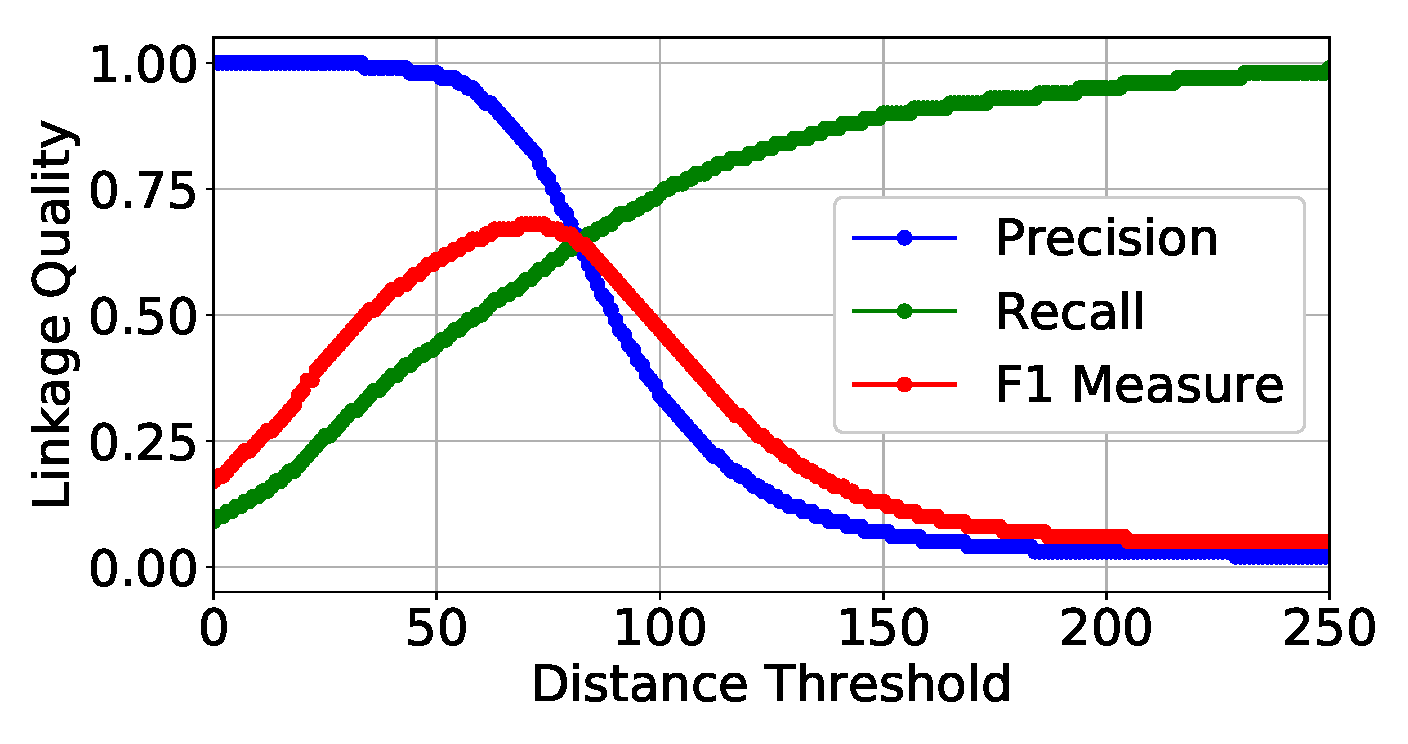
\includegraphics[width=\textwidth]{figures/plotLQ-cora-brute}
\caption{Cora - Brute Force}
\end{subfigure}%
\begin{subfigure}{.5\textwidth}
  \centering
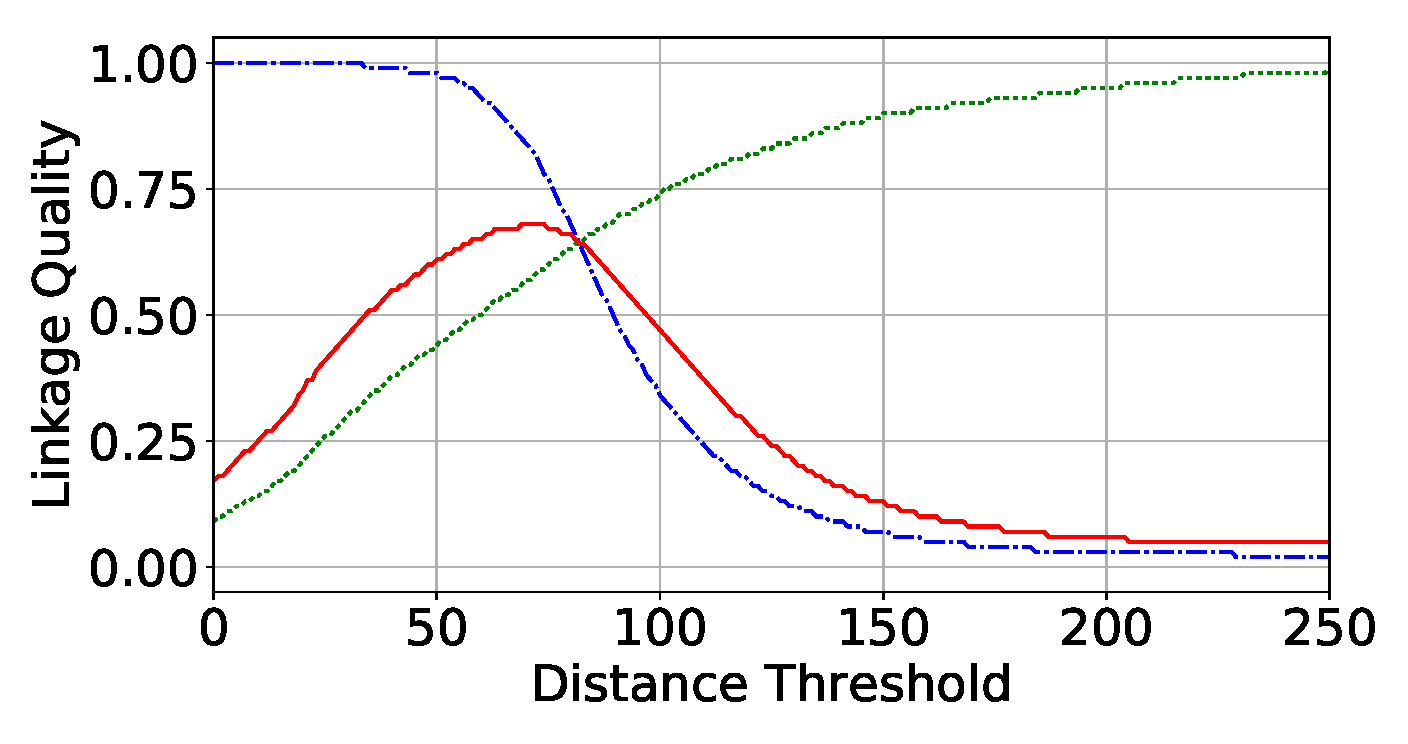
\includegraphics[width=\textwidth]{figures/plotLQ-cora-mtree}
\caption{Cora - M-tree}
\end{subfigure}

\begin{subfigure}{.5\textwidth}
  \centering
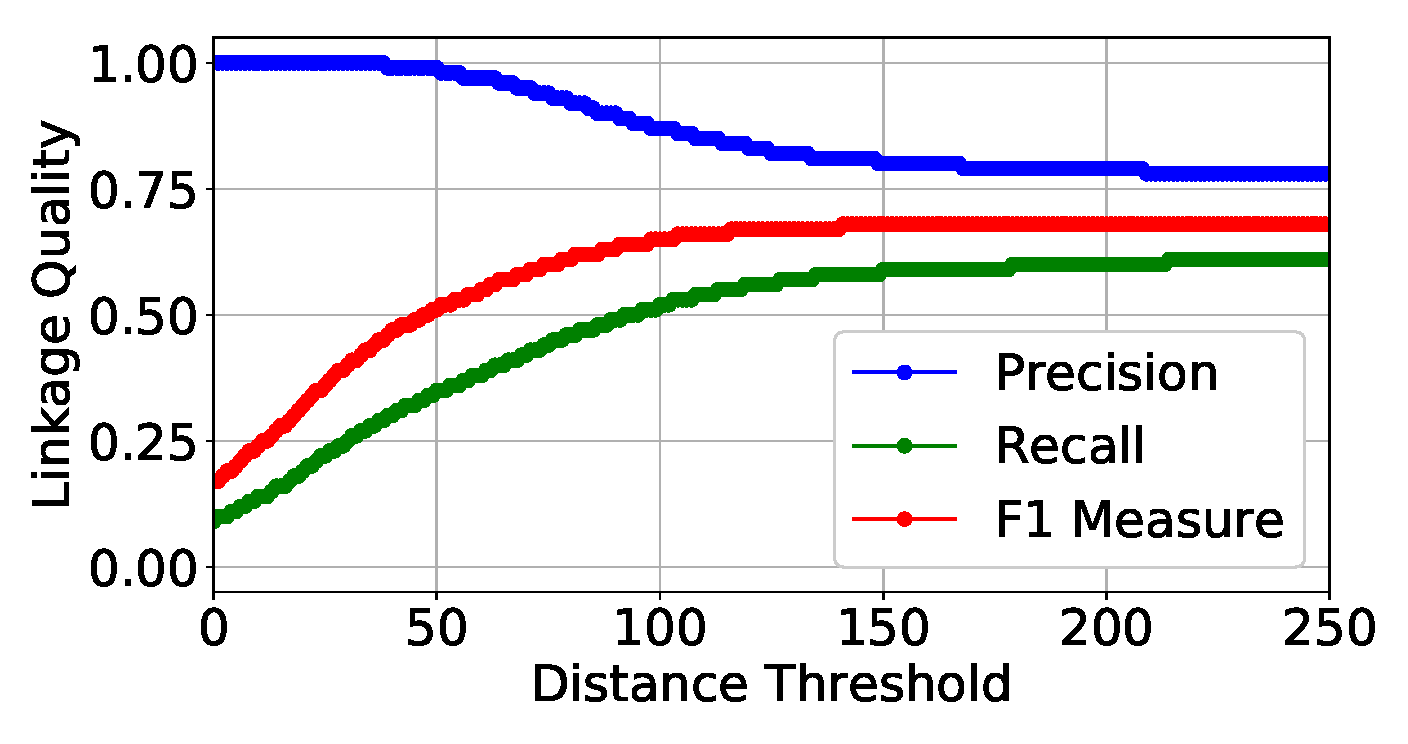
\includegraphics[width=\textwidth]{figures/plotLQ-cora-trad-authors}
\caption{Cora - Traditional Blocking on the `authors' field}
\end{subfigure}%
\begin{subfigure}{.5\textwidth}
  \centering
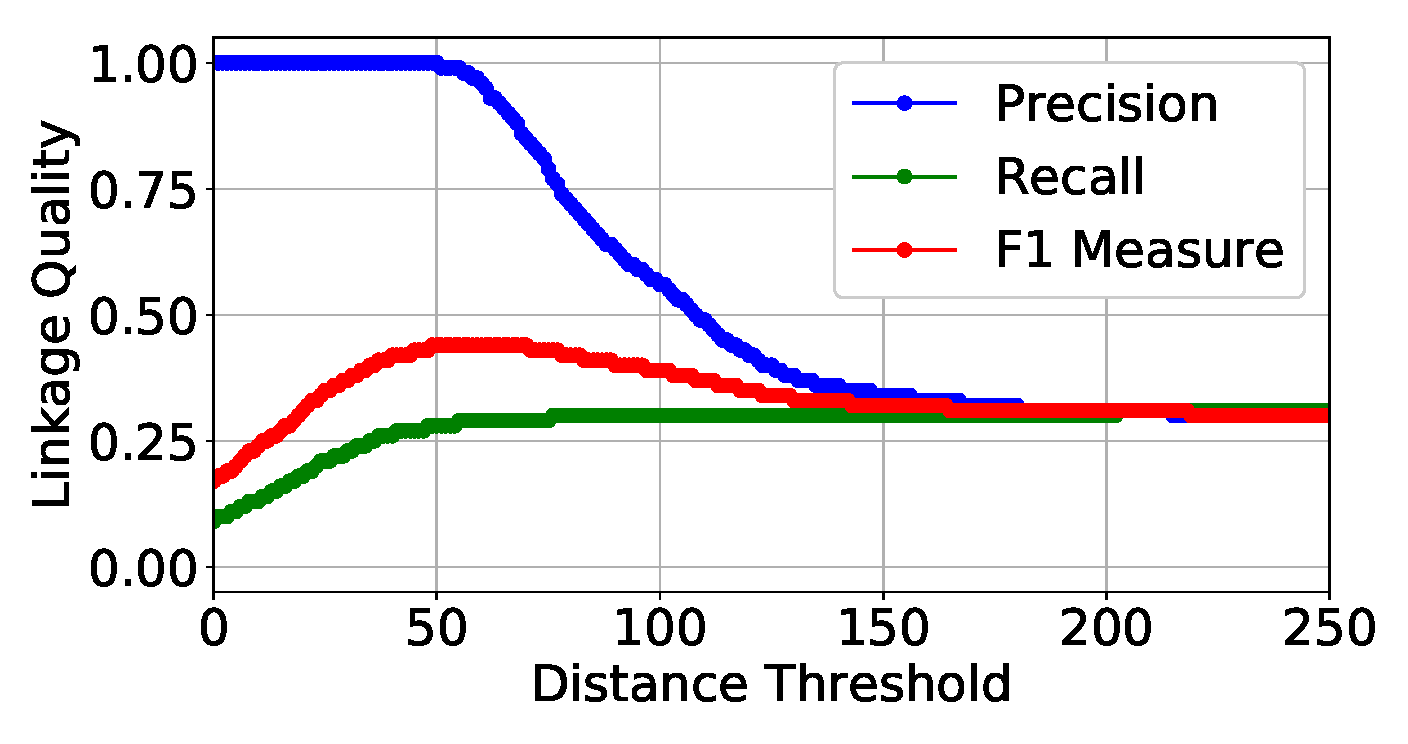
\includegraphics[width=\textwidth]{figures/plotLQ-cora-trad-title}
\caption{Cora - Traditional Blocking on the `title' field}
\end{subfigure}

\begin{subfigure}{.5\textwidth}
  \centering
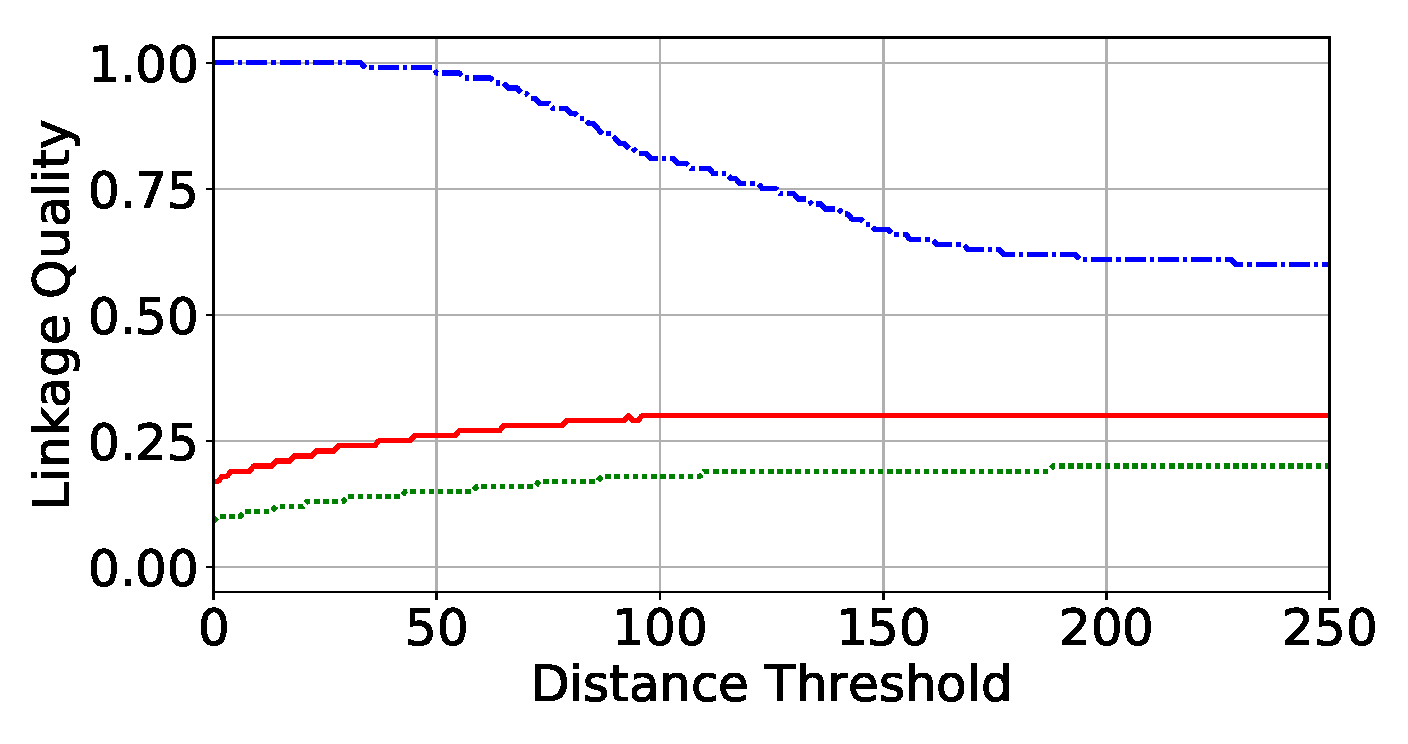
\includegraphics[width=\textwidth]{figures/plotLQ-cora-trad-year}
\caption{Cora - Traditional Blocking on the `publication year' field}
\end{subfigure}%
\begin{subfigure}{.5\textwidth}
  \centering
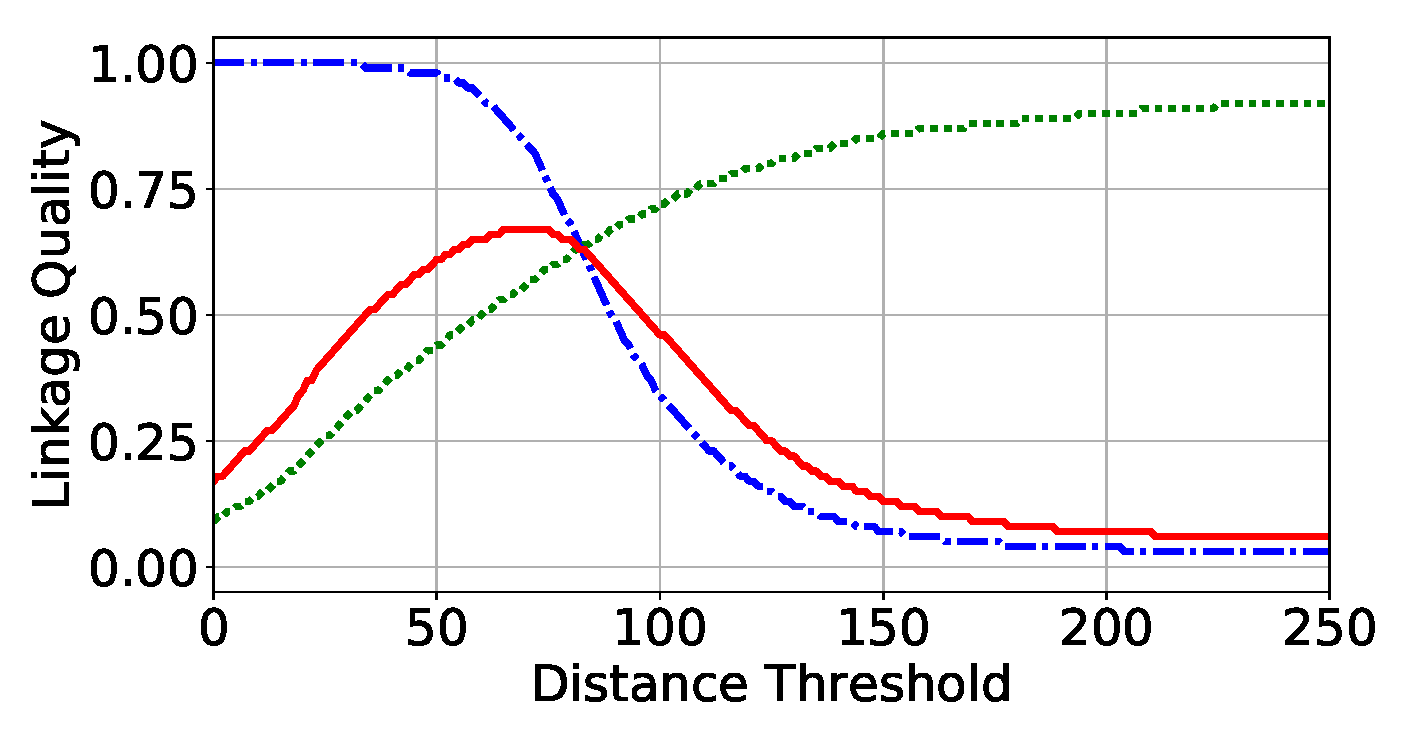
\includegraphics[width=\textwidth]{figures/plotLQ-cora-trad-combined}
\caption{Cora - Traditional Blocking using the union of blocking on all fields}
\end{subfigure}

\begin{subfigure}{.5\textwidth}
  \centering
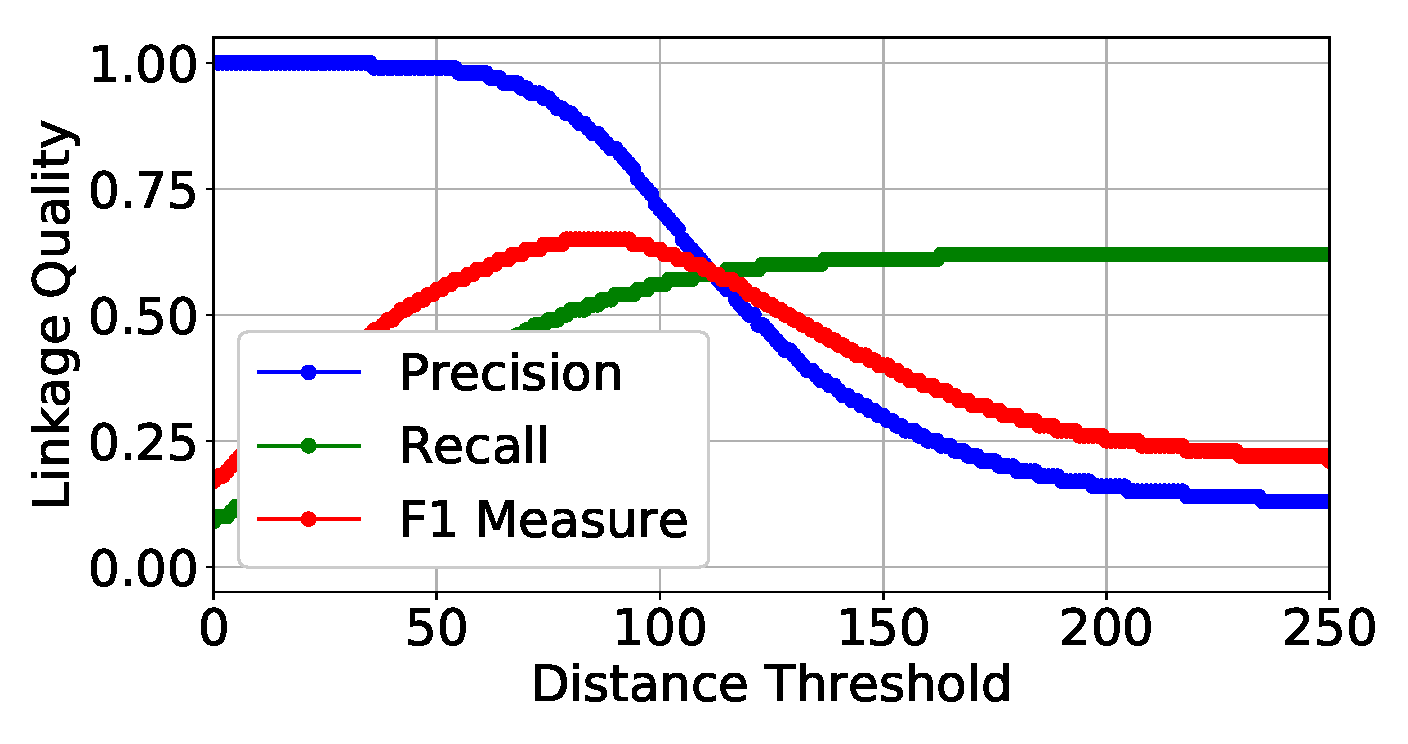
\includegraphics[width=\textwidth]{figures/plotLQ-cora-lsh-2-2}
\caption{Cora - LSH Blocking using 2 bands of size 2}
\end{subfigure}%
\begin{subfigure}{.5\textwidth}
  \centering
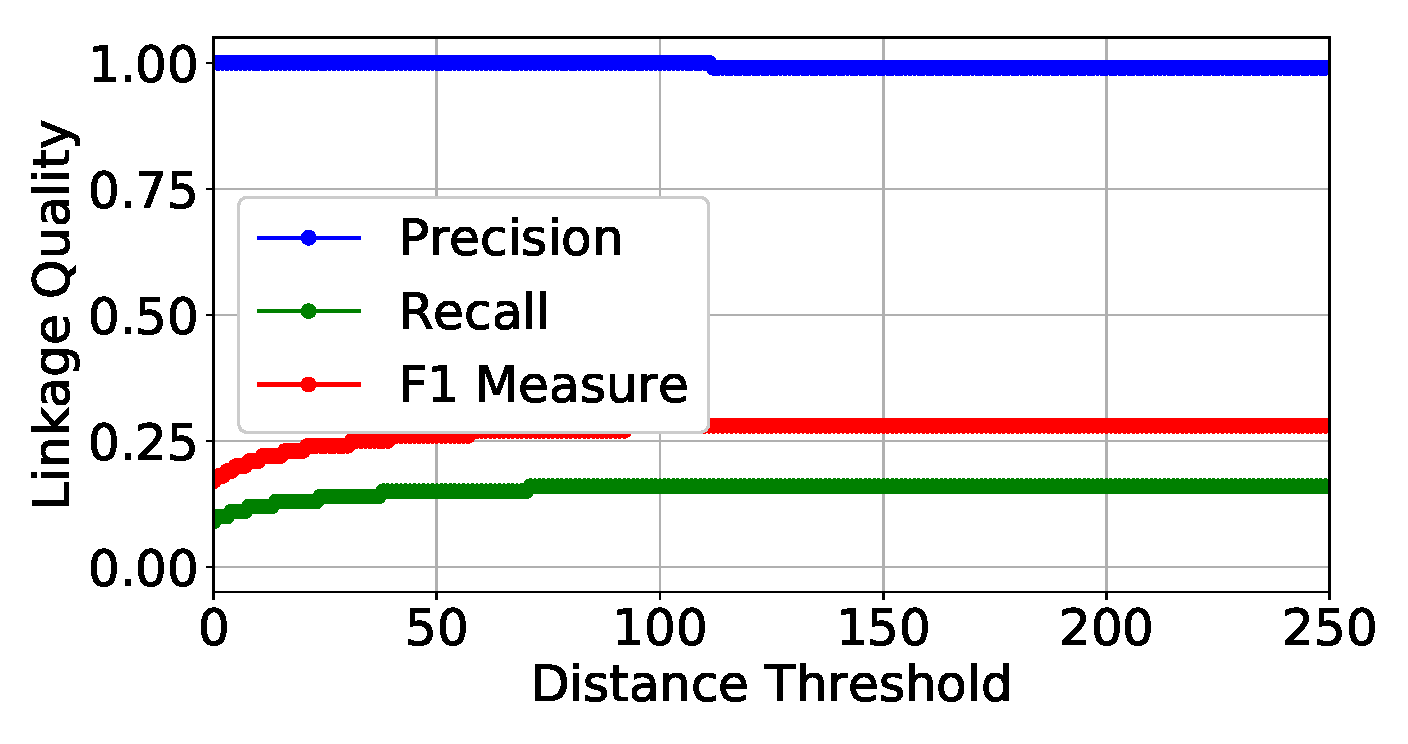
\includegraphics[width=\textwidth]{figures/plotLQ-cora-lsh-2-10}
\caption{Cora - LSH Blocking using 2 bands of size 10}
\end{subfigure}

\begin{subfigure}{.5\textwidth}
  \centering
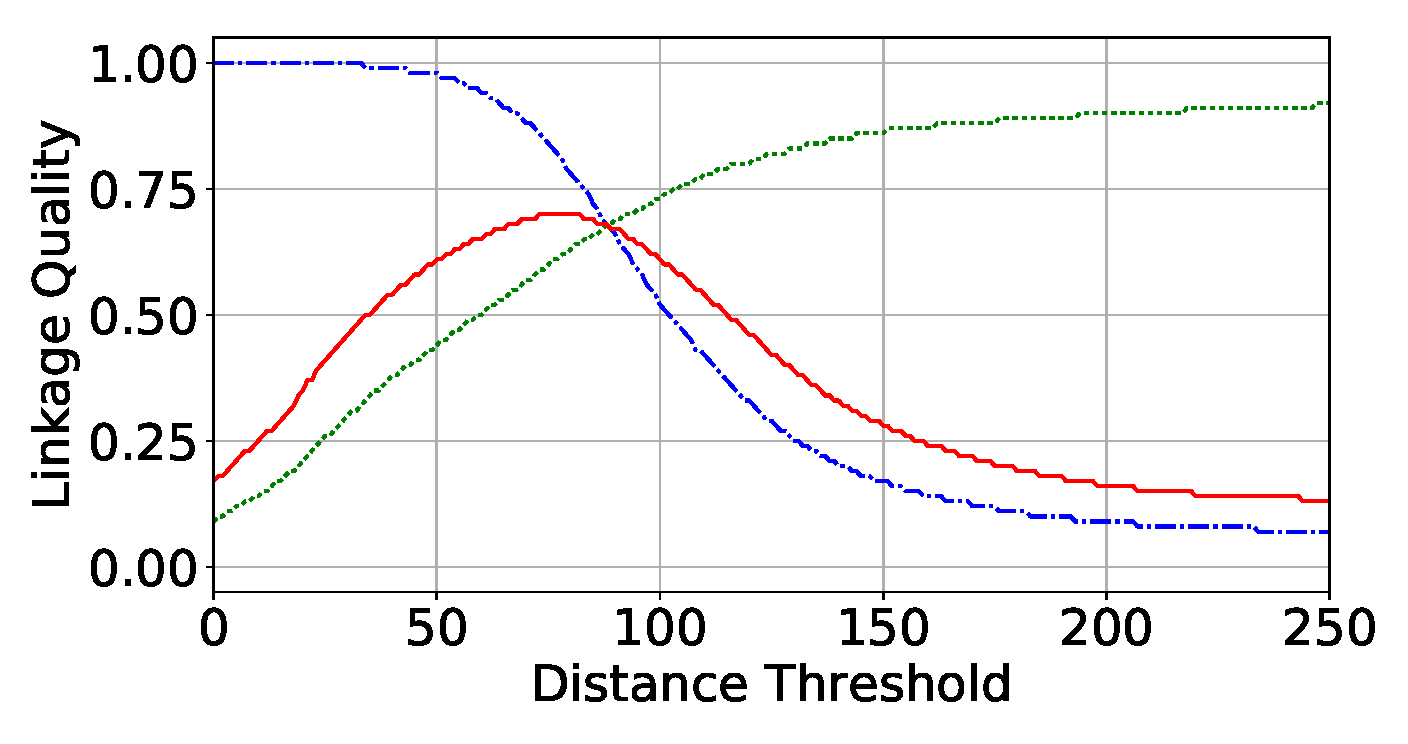
\includegraphics[width=\textwidth]{figures/plotLQ-cora-lsh-10-2}
\caption{Cora - LSH Blocking using 10 bands of size 2}
\end{subfigure}%
\begin{subfigure}{.5\textwidth}
  \centering
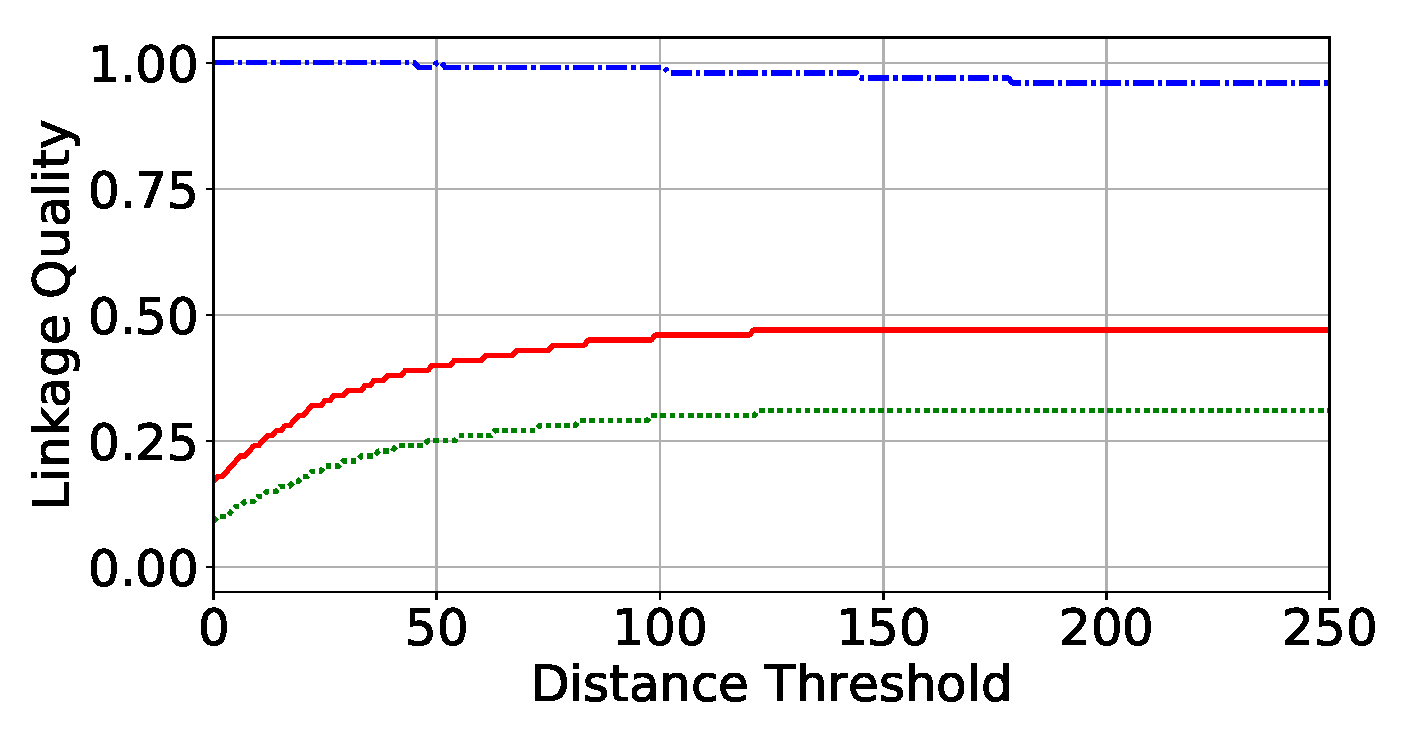
\includegraphics[width=\textwidth]{figures/plotLQ-cora-lsh-10-10}
\caption{Cora - LSH Blocking using 10 bands of size 10}
\end{subfigure}

\caption{Linkage results on the Cora data set}
\label{cora-quality}
\end{figure}

% \begin{figure}
% 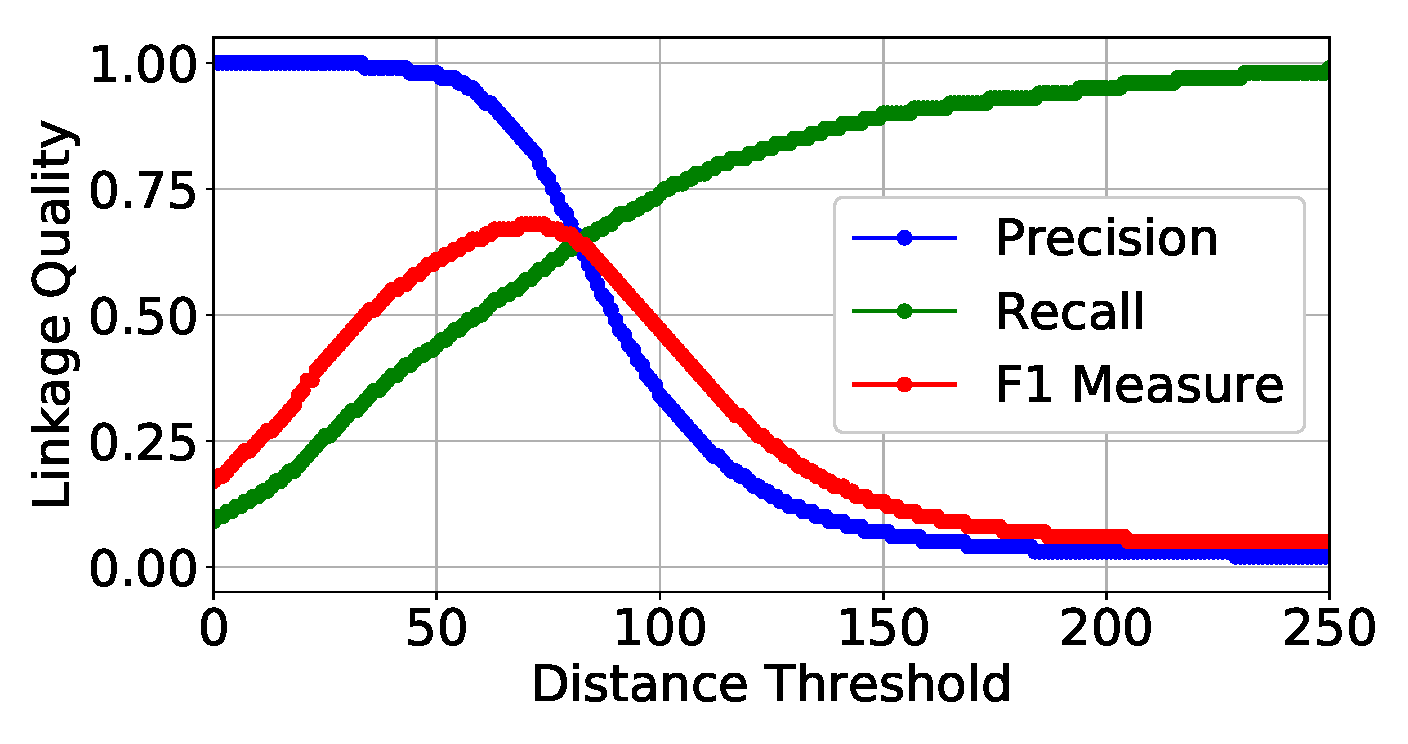
\includegraphics[width=\textwidth]{figures/plotLQ-cora-brute}
% \caption{Linkage quality using brute-force linking on the Cora dataset\label{fig-cora-brute}}
% \end{figure}

In the traditional blocking experiment the following fields from the
Cora dataset are used individually as blocking keys: \textit{author},
\textit{title}, \textit{venue}, \textit{location}, \textit{publisher}
and \textit{year}. We also use a combined blocking key comprising all
fields.

\Cref{comparison-of-results-cora} shows greater detail for a subset of
the Cora experiments, with the distance threshold fixed at 70. The table
shows the parameters for the experiment, the number of distance
comparisons made, the precision, recall and the F1 measure achieved by
each algorithm.  In the \emph{Linker} column the algorithm name is
followed by its parameters: for LSH the number of the bands followed by
the band size, and for traditional blocking the fields used for
blocking. The number of distance comparisons is reported as a
machine-independent proxy for execution cost, since code profiling shows
that distance calculations are dominant.

M-tree yields the same linkage quality as brute-force, although using a significantly lower
number of comparisons. This is as expected, since both techniques are complete.

Three of the LSH configurations give qul


\begin{table}[ht]
\centering
\begin{tabular}{l|r|r|r|r}
\parbox{0.2\textwidth}{\centering Linker} &
\parbox{0.2\textwidth}{\centering Comparisons} &
\parbox{0.17\textwidth}{\centering Precision} &
\parbox{0.17\textwidth}{\centering Recall} &
\parbox{0.17\textwidth}{\centering F1 Measure} \\ \hline \hline
Brute Force        & 1,677,025                 & 0.84      & 0.57   & 0.68       \\ \hline
MTree              &  902,693                  & 0.84      & 0.57   & 0.68       \\ \hline
LSH-2-2            &  192,199	& 0.95	& 0.47	& 0.63       \\
LSH-5-2            &  342,849	& 0.91	& 0.55	& 0.69       \\
LSH-10-2           &  513,947	& 0.88	& 0.57	& 0.69       \\
LSH-2-5            &  14,329	& 0.99	& 0.28	& 0.43      \\
LSH-5-5            &  22,057	& 0.99	& 0.36	& 0.53       \\
LSH-10-5           &  26,167	& 0.98	& 0.4	& 0.57      \\
LSH-2-10           &  4,711	& 1	& 0.15	& 0.27    \\
LSH-5-10           &  6,501	& 1	& 0.19	& 0.32      \\
LSH-10-10          & 10,627  	& 0.99	& 0.27& 	0.43       \\  \hline
Block-year         &  115,893                  & 0.99      & 0.35   & 0.51       \\
Block-authors      &   11,039                   & 0.94      & 0.16   & 0.28       \\
Block-title        &   27,407                   & 0.95      & 0.42   & 0.58       \\
Block-venue        &   36,647                   & 0.85      & 0.29   & 0.44       \\
Block-location     & 1,009,957                 & 0.83      & 0.43   & 0.57       \\
Block-publisher    &  833,079                  & 0.85      & 0.44   & 0.58       \\
Block-combined     & 1,214,269                 & 0.84      & 0.56   & 0.67       \\ \hline
\end{tabular}
\caption{Linkage quality on Cora dataset with distance threshold = 70
\label{comparison-of-results-cora}
}
\end{table}

\subsection{Historical Demography results}

\Cref{comparison-of-results-demography-skye} and \Cref{comparison-of-results-demography-kili} show the results for LSH-Minhash and M-tree on the Skye and Kilmarnock datasets. Linkage was performed between birth and death records. The shingle size was set to 2 for all the LSH experiments reported, as this was found to give good results and LSH was not especially sensitive to this parameter. Results for other shingle sizes were omitted from this paper for brevity. In both cases the F1 measure achieved is better for M-tree than any of the experimental settings chosen for LSH. This is largely due to the recall for M-tree being much higher than any of the LSH experiments. For all LSH parameters LSH out performs M-tree in terms of precision.

Perhaps more important than the fact that M-tree gives better F1 measures than all of the LSH experiments is the fact that the LSH performance is extremely variable. For a relatively plausible settings for the number of bands and band-size the F1 measurements vary from 0.01 (extremely poor) to 0.47 (relatively good) for Skye and between 0.03 and 0.49 for the Kilmarnock dataset. In both cases LSH-10-2 performs best, but since this is data dependent there is no guarantee these parameters would work well with another dataset. Furthermore, without good ground truth, which is usually unavailable, there is no way of knowing if good linkage results are being obtained or not.

Another observation that is worthy of comment is the number of (distance) comparisons being performed by the different algorithms. For M-trees the number of comparisons are closely related to the complexity of the search being performed since the algorithms are performing (range) searches over distance measures to determine the query results. This is not true of LSH which is performing Jaccard similarity using Hashes over the datasets. Comparisons are only used at the final step to determine if a candidate is a match or not. The LSH results which provide the best results by F1 measure are performing between a quarter and half the number of matches performed by M-trees. From this we can conclude that the hash algorithms are returning many candidates that are outwith the search distance. Thus, in order to get good results, LSH is tending towards a brute force search over the candidate results. Despite this LSH is much faster due to the efficiency of the hashing mechanisms.

\begin{table}[ht]
\centering
\begin{tabular}{l|r|r|r|r}
\parbox{0.2\textwidth}{\centering Linker} &
\parbox{0.2\textwidth}{\centering Comparisons} &
\parbox{0.17\textwidth}{\centering Precision} &
\parbox{0.17\textwidth}{\centering Recall} &
\parbox{0.17\textwidth}{\centering F1 Measure} \\ \hline \hline
MTree    & 102,318,525                 & 0.65      & 0.46   & 0.54      \\ \hline

LSH-2-2  & 3,109,250                   & 0.63      & 0.03   & 0.06       \\

LSH-5-2  & 10,412,496                  & 0.64      & 0.11   & 0.19       \\

LSH-10-2 & 53,874,127                  & 0.68      & 0.36   & 0.47       \\

LSH-5-5  & 36,566                     & 0.76      & 0.01   & 0.01       \\

LSH-10-5 & 129,873                    & 0.72      & 0.01   & 0.02       \\ \hline
\end{tabular}
\caption{Linkage quality on Skye dataset with distance threshold = 2
\label{comparison-of-results-demography-skye}
}
\end{table}

%-------------------------------------------------------------------------------------

\begin{table}[ht]
\centering
\begin{tabular}{l|r|r|r|r|r|r}
\parbox{0.2\textwidth}{\centering Linker} &
\parbox{0.2\textwidth}{\centering Comparisons} &
\parbox{0.17\textwidth}{\centering Precision} &
\parbox{0.17\textwidth}{\centering Recall} &
\parbox{0.17\textwidth}{\centering F1 Measure} \\ \hline \hline
MTree     & 514,871,153                   & 0.76      & 0.45   & 0.57      \\ \hline
LSH-2-2   & 99,145,887                    & 0.81      & 0.16   & 0.27       \\
LSH-5-2   & 130,721,338                   & 0.79      & 0.23   & 0.36       \\
LSH-10-2  & 177,168,848                   & 0.79      & 0.36   & 0.49       \\
LSH-5-5   & 239,368                      & 0.84      & 0.01   & 0.02       \\
LSH-10-5  & 855,431                      & 0.87      & 0.02   & 0.03 \\ \hline
\end{tabular}
\caption{Linkage quality on Kilmarnock dataset with distance threshold = 2
\label{comparison-of-results-demography-kili}
}
\end{table}

%-------------------------------------------------------------------------------------

\begin{figure}
\centering
\begin{subfigure}{.5\textwidth}
  \centering
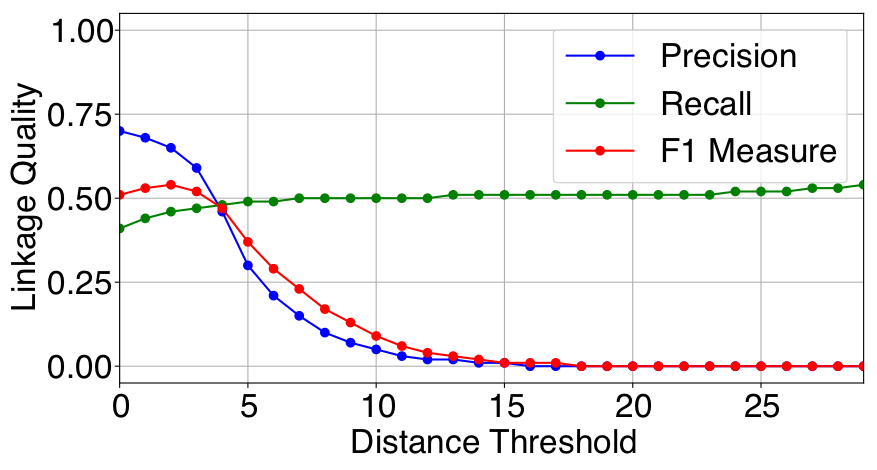
\includegraphics[width=\textwidth]{figures/skye-mtree}
\caption{Linkage quality on Skye dataset using M-tree\label{skye-quality-mtree}}
\end{subfigure}%
\begin{subfigure}{.5\textwidth}
  \centering
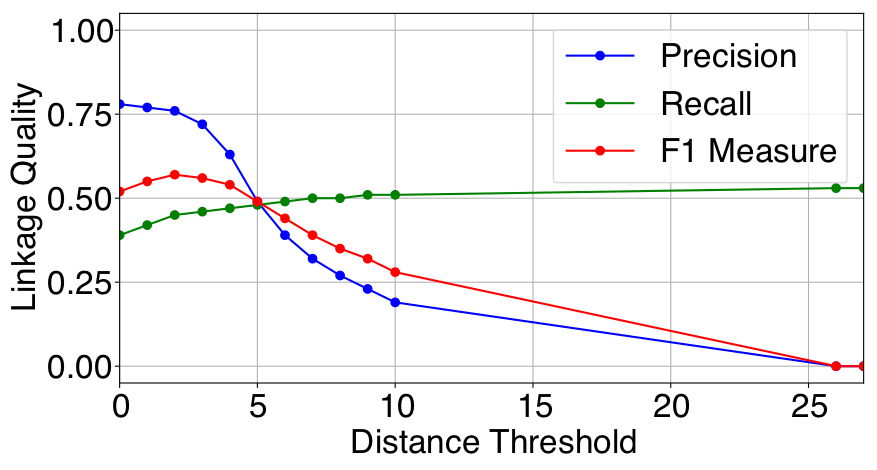
\includegraphics[width=\textwidth]{figures/kili-mtree}
\caption{Linkage quality on Kilmarnock dataset using M-tree\label{kilmarnock-quality-mtree}}
\end{subfigure}

\begin{subfigure}{.5\textwidth}
  \centering
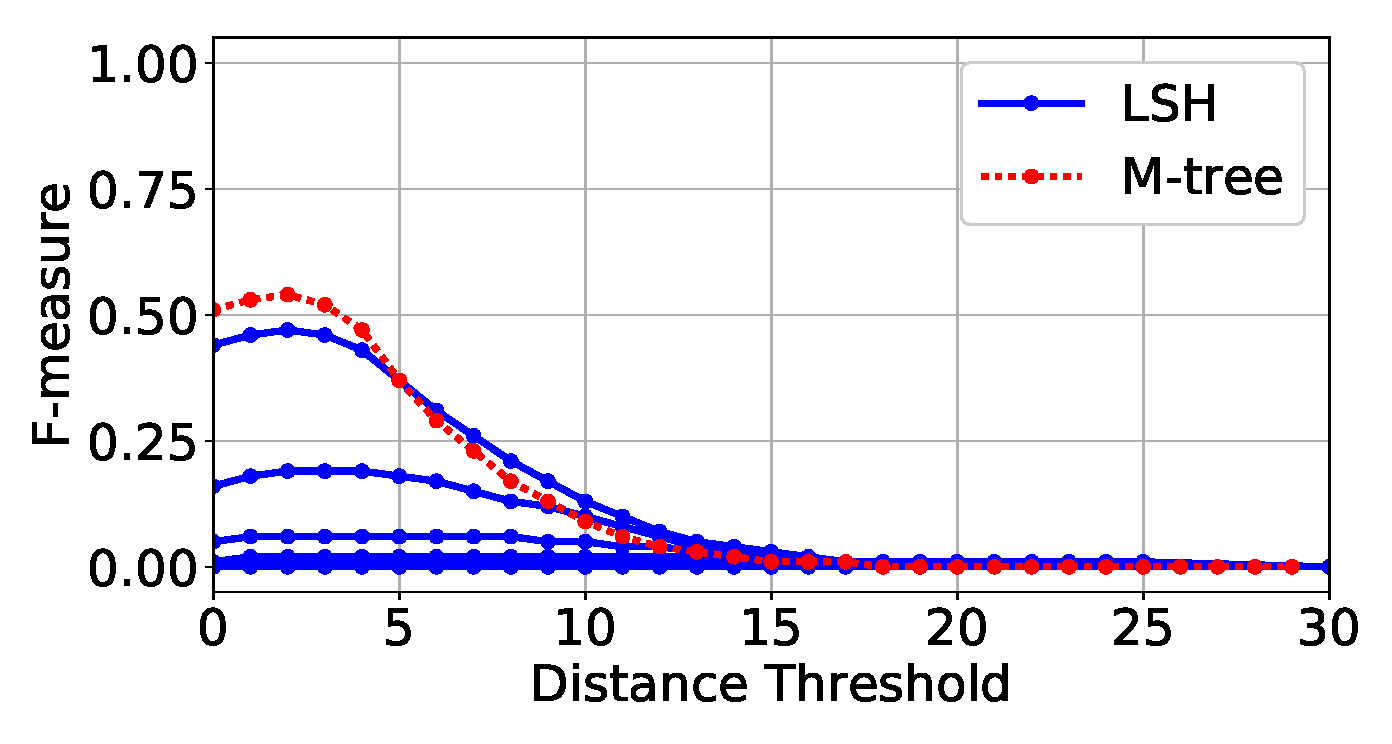
\includegraphics[width=\textwidth]{figures/plotFs-skye-f}
\caption{Linkage quality on Skye dataset using M-tree and all LSH configurations}
\end{subfigure}%
\begin{subfigure}{.5\textwidth}
  \centering
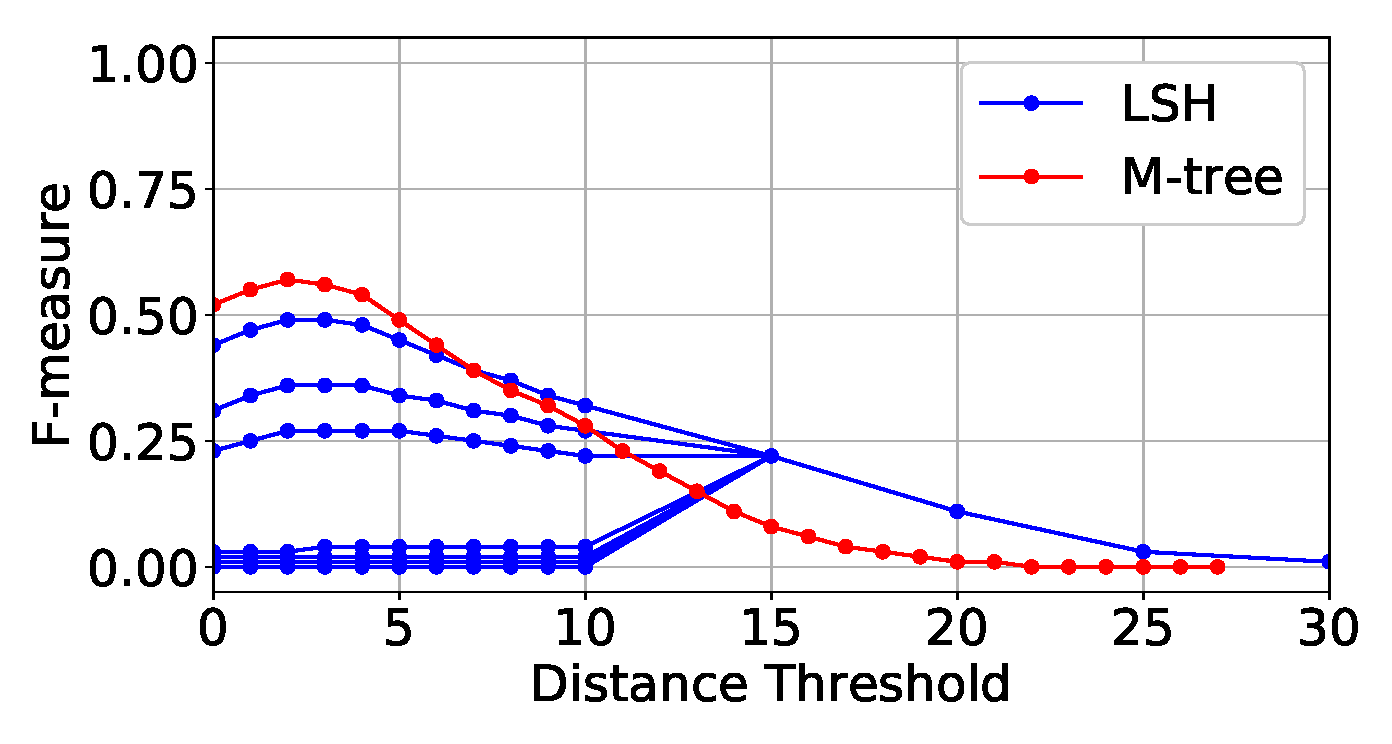
\includegraphics[width=\textwidth]{figures/plotFs-kilmarnock-f}
\caption{Linkage quality on Kilmarnock dataset using M-tree and all LSH configurations}
\end{subfigure}

\caption{Linkage results on the demographic datasets}
\label{demography-quality-mtree}
\end{figure}

% --------------------------------------------------------------------

\section{Conclusions and Future Work\label{sec-concl}}

In this paper we have demonstrated the efficacy of MSI in achieving  complete and efficient record linkage, without the need for complex parameter tuning. In conclusion, this assertion deserves some careful unpacking. It is always possible to achieve high quality linkage using a brute-force approach. However the n-squared complexity of this approach prevents its practical application for datasets of even moderate size. The use of MSI techniques such as M-tree delivers the same results as the brute-force approach with fewer comparisons. We have shown that the M-tree approach delivers high precision, high recall results that are the same as those delivered by the brute-force approach. Furthermore this is achieved consistently without the need for complex parameter tuning.

We contrast this to traditional blocking and LSH based approaches. The major drawback of their use is that whilst they can produce extremely good results, they can also produce extremely poor results. It was our observations of low recall given by these approaches that originally led us to experiment with M-trees. Without extensive ground truth or large amounts of clerking effort by human domain experts it is impossible to determine the quality of the links produced. 

However, this paper also highlights some unexpected results. Firstly, the good quality results yielded by both traditional blocking and LSH are partly due to the fact that (in the limit) they tend towards brute-force as the number of records in the block increase. A second unexpected result is that shown in \Cref{quality-cora}, namely that LSH can yield higher precision than is achieved by a complete method such as M-tree, as was discussed in Sect.~\ref{sec-approach}.


\emph{Some sentence or two about run-time?}

The observation that LSH can yield results quickly at the cost of some recall suggests a potentially profitable future direction for exploration, namely the use of hybrid algorithms. We hypothesise that it may be possible to use an incomplete technique like LSH to form indices into a data structure such as an M-tree. In this manner, M-tree nodes could be used as the starting point for range-search queries and, in so doing, prune the search space considerably to yield highly quality complete results quickly.

% TODO: check that the above claims have been addressed.

% --------------------------------------------------------------------

\bibliographystyle{splncs03}
\bibliography{paper.bib} 

% ====================================================================

\end{document}

% ====================================================================

%text cut from earlier versions:

%The MIFile \cite{amato2014mi} approach is an inexact technique for performing similarity search based on metric spaces. Using  MI\_file,  each record is represented by the ordering of distances from a collection of reference objects.
% Peter: are these reference object also records? 
It is based on the idea that two records close to each other will have similar neighbours and will thus be represented by similar of distances
% Peter: unclear what you mean with: similar of distances
from the chosen reference objects. 
In order to create the indexes, for each value to be added to the
% peter: value -> record ?
data-structure, first the k nearest reference objects (governed by a fixed parameter) are found, each is given a score (drawn from 1,2,3... based on the reference object's position from the value).
% peter: this is unclear .. I think I understand k-NN: for each
% record you find the k nearest reference objects and you enumerate
% them
Next for each score, a  mapping is created in an inverted index mapping
% peter: unclear..? a mapping in an inverted index mapping?
from the value to the score of each reference object and a representation of the data associated with the reference object and the value inserted.
% peter: unclear: what is "the data" associated with the reference
% object.
In order to perform a \textit{nearest-neighbour} lookup, first the k nearest reference objects (bounded by a second fixed parameter).
% peter: this sentence reads incomplete..?
Next the objects closest to these reference objects are extracted from the inverted map by choosing the neighbours with the highest score.
% Peter: sorry, this is unclear as well. "the objects closest" ->
% records closest? And why highest scores..? Is the closest record
% to a reference object given the highest score (not the lowest
% score - i.e. not 1-closest, 2-closest etc)
Much of the search space may be eliminated by  keeping track of the scores that  can contribute to the nearest neighbours.
% peter: so I guess you use the triangular inequality and the reference
% objects to prune the search space.


\cite{Yu2016} surveys the use of string similarity in record linkage.
Algorithms used to compare two records are characterised as being
character-based or token-based. The first category, including approaches
such as Levenshtein~\cite{Levenshtein66}, uses character differences in
the strings being compared. The second, including techniques such as
Jaccard similarity, treats records as sets of tokens, and utilises set
similarity. There are also hybrids of the two approaches.
% Do we need the rest of this paragraph?
\cite{Yu2016} categorises linkage algorithms as being based on filtering,
verification, or thresholds.
% This is missing some context as to what is going on.
Filtering algorithms generate signatures for each record, construct
inverted lists containing records with common signatures, and prune
records with no common signatures.
% Distance of prefix to what? What is the data in this context?
Verification algorithms calculate the exact distances of a prefix of the
data, and use another technique to estimate the edit distance between
records. If the estimated distance is larger than the desired similarity
threshold, the candidate may be discarded.
% This seems a bit throw-away.
% Also, these aren't themselves linkage algorithms are they?
Threshold-based algorithms include M-trees, Trie-Join, Pass-Join and
Partenum.

%We will evaluate the performance of LSH based blocking with regard to the three parameters $l_{ss}$, $l_{bs}$ and $l_{nb}$ in
Sect.~\ref{sec-exp}.


% \begin{table}[t]
% \caption{Parameter settings used for the different datasets used in
%    the experiments,with $d$ the distance threshold used, $l_{ss}$, $l_{sb}$ and $l_{nb}$ the LSH
%    shingle size, and the size and number of bands, respectively.}
%  \label{table-parameters}
%   \centering
%   \begin{scriptsize}
%   %\addtolength{\tabcolsep}{-0.5pt}
%   \begin{tabular}{ccccc}
%   \hline\noalign{\smallskip}
%   Dataset~ & $d$ & $l_{ss}$ & $l_{bs}$ & $l_{nb}$ \\
%   name(s) & & & &  \\
%   \noalign{\smallskip} \hline \noalign{\smallskip}
%   CORA & ~$[0,5,10,\ldots,95,100]$~ & ~$2$~ &
%     ~$[2,5,10]$~ & ~$[2,5,10]$~  \\
%   Isle of Skye &  \\
%   Kilmarnock  &  \\
%   \noalign{\smallskip} \hline
%   \end{tabular}
%   \end{scriptsize}
% \end{table}

% \textbf{Experimental Setup:}
% %
% We implemented all techniques described in Sect.~\ref{sec-approach}
% using Java (version 1.8.0\_144) and ran an extensive set of experiments on
% a compute server with 24 Intel(R) Xeon(R) processors running at 2.30GHz, 
% 128 GBytes of main memory and running Red Hat 4.8.5-11.


